\documentclass[a4paper,12pt]{article}
\usepackage{amsmath}
\usepackage{hyperref}
\usepackage{graphicx}
\usepackage{float}
\usepackage{subcaption}
\usepackage{listings}
\usepackage{circuitikz}

\title{Lab Report 5: Op-Amp Applications}
\author{Arnav Yadnopavit- EE24BTECH11007\\Prajwal - EE24BTECH11051}
\date{\today}

\begin{document}

\maketitle

\section*{Objective}
To study the applications of operational amplifiers (Op-Amps) by implementing:
\begin{itemize}
    \item Custom weighted summing and difference amplifier
    \item Op-Amp integrator
    \item Precision rectifier (Super Diode)
\end{itemize}

\section*{Apparatus}
\begin{itemize}
    \item Operational Amplifiers (LM358)
    \item Resistors (selected for proper weighting and circuit operation)
    \item Capacitors (for integration circuit)
    \item Diodes (e.g., 1N4148 for rectification)
    \item DC power supply
    \item Function generator
    \item Oscilloscope
\end{itemize}

\section*{Theory}
\subsection*{1. Custom Weighted Summing and Difference Amplifier}
A summing amplifier combines multiple inputs with specified gains:
\begin{equation}
V_{out} = -\left(\frac{R_f}{R_1}V_1 + \frac{R_f}{R_2}V_2 \right)
\end{equation}
$R_1=R_2=2k\Omega$, $R_3=1k\Omega$
\begin{equation}
V_{out} = \frac{V_1 + V_2}{2}
\end{equation}
\begin{figure}[H]
    \centering
    
\begin{circuitikz}
\tikzstyle{every node}=[font=\large]

\draw (12.75,11.25) node[op amp,scale=1, yscale=-1 ] (opamp2) {};
\draw (opamp2.+) to[short] (11.25,11.75);
\draw  (opamp2.-) to[short] (11.25,10.75);
\draw (13.95,11.25) to[short](14.25,11.25);
\draw (11.25,11.75) to (10.75,11.75) node[ground]{};
\draw (8.25,9.25) to[R] (10.25,9.25);
\draw (9.25,7.5) to[R] (11.25,7.5);
\draw (11.25,7.5) to[short] (11.25,10.75);
\draw (10.25,9.25) to[short] (11.25,9.25);
\draw (8,7.5) to[sinusoidal voltage source, sources/symbol/rotate=auto] (9.25,7.5);
\draw (6.75,9.25) to[sinusoidal voltage source, sources/symbol/rotate=auto] (8.25,9.25);
\draw (11.25,9.25) to[R] (13.25,9.25);
\draw (13.25,9.25) to[short] (13.75,9.25);
\draw (13.75,9.25) to[short] (13.75,11.25);
\node at (11.25,9.25) [circ] {};
\node at (13.75,11.25) [circ] {};
\draw (12.75,11.25) node[op amp,scale=1, yscale=-1 ] (opamp2) {};
\draw (opamp2.+) to[short] (11.25,11.75);
\draw  (opamp2.-) to[short] (11.25,10.75);
\draw (13.95,11.25) to[short](14.25,11.25);
\draw (6.75,9.25) to (6.75,8.75) node[ground]{};
\draw (8,7.5) to (8,7) node[ground]{};
\draw (14.25,11.25) to[short, -o] (16.25,11.25) ;
\node [font=\large] at (6.75,10.25) {$V_1$};
\node [font=\large] at (8.25,8.25) {$V_2$};
\node [font=\large] at (9.25,10) {$R_1$};
\node [font=\large] at (10.25,8.25) {$R_2$};
\node [font=\large] at (12.25,9.75) {$R_f$};
\node [font=\large] at (16,11.75) {$V_{out}$};
\end{circuitikz}
    \caption{Summing and Difference Amplifier Circuit}
\end{figure}

\subsection*{2. Op-Amp Integrator}
The Op-Amp integrator performs mathematical integration:
\begin{equation}
V_{out} = -\frac{1}{RC} \int V_{in} dt
\end{equation}
It converts a square wave input into a triangular wave output and is useful in signal processing applications.
\begin{figure}[H]
    \centering
    
\begin{circuitikz}
\tikzstyle{every node}=[font=\large]

\draw (12.75,11.25) node[op amp,scale=1, yscale=-1 ] (opamp2) {};
\draw (opamp2.+) to[short] (11.25,11.75);
\draw  (opamp2.-) to[short] (11.25,10.75);
\draw (13.95,11.25) to[short](14.25,11.25);
\draw (11.25,11.75) to (10.75,11.75) node[ground]{};
\draw (8.25,9.25) to[R] (10.25,9.25);
\draw (9.25,7.5) to[R] (11.25,7.5);
\draw (11.25,7.5) to[short] (11.25,10.75);
\draw (10.25,9.25) to[short] (11.25,9.25);
\draw (8,7.5) to[sinusoidal voltage source, sources/symbol/rotate=auto] (9.25,7.5);
\draw (6.75,9.25) to[sinusoidal voltage source, sources/symbol/rotate=auto] (8.25,9.25);
\draw (11.25,9.25) to[R] (13.25,9.25);
\draw (13.25,9.25) to[short] (13.75,9.25);
\draw (13.75,9.25) to[short] (13.75,11.25);
\node at (11.25,9.25) [circ] {};
\node at (13.75,11.25) [circ] {};
\draw (12.75,11.25) node[op amp,scale=1, yscale=-1 ] (opamp2) {};
\draw (opamp2.+) to[short] (11.25,11.75);
\draw  (opamp2.-) to[short] (11.25,10.75);
\draw (13.95,11.25) to[short](14.25,11.25);
\draw (6.75,9.25) to (6.75,8.75) node[ground]{};
\draw (8,7.5) to (8,7) node[ground]{};
\draw (14.25,11.25) to[short, -o] (16.25,11.25) ;
\node [font=\large] at (6.75,10.25) {$V_1$};
\node [font=\large] at (8.25,8.25) {$V_2$};
\node [font=\large] at (9.25,10) {$R_1$};
\node [font=\large] at (10.25,8.25) {$R_2$};
\node [font=\large] at (12.25,9.75) {$R_f$};
\node [font=\large] at (16,11.75) {$V_{out}$};
\end{circuitikz}
    \caption{Op-Amp Integrator Circuit}
\end{figure}
\subsection*{3. Precision Rectifier (Super Diode)}
A precision rectifier eliminates the 0.7V drop of standard diodes by using an Op-Amp:
\begin{equation}
V_{out} = \begin{cases} 0, & V_{in} < 0 \\ V_{in}, & V_{in} > 0 \end{cases}
\end{equation}
For a full-wave rectifier, an additional summing stage is used.
\subsection*{Precision Rectifier}
\begin{figure}[H]
    \centering
    
\begin{circuitikz}
\tikzstyle{every node}=[font=\large]

\draw (12.75,11.25) node[op amp,scale=1, yscale=-1 ] (opamp2) {};
\draw (opamp2.+) to[short] (11.25,11.75);
\draw  (opamp2.-) to[short] (11.25,10.75);
\draw (13.95,11.25) to[short](14.25,11.25);
\draw (11.25,11.75) to (10.75,11.75) node[ground]{};
\draw (8.25,9.25) to[R] (10.25,9.25);
\draw (9.25,7.5) to[R] (11.25,7.5);
\draw (11.25,7.5) to[short] (11.25,10.75);
\draw (10.25,9.25) to[short] (11.25,9.25);
\draw (8,7.5) to[sinusoidal voltage source, sources/symbol/rotate=auto] (9.25,7.5);
\draw (6.75,9.25) to[sinusoidal voltage source, sources/symbol/rotate=auto] (8.25,9.25);
\draw (11.25,9.25) to[R] (13.25,9.25);
\draw (13.25,9.25) to[short] (13.75,9.25);
\draw (13.75,9.25) to[short] (13.75,11.25);
\node at (11.25,9.25) [circ] {};
\node at (13.75,11.25) [circ] {};
\draw (12.75,11.25) node[op amp,scale=1, yscale=-1 ] (opamp2) {};
\draw (opamp2.+) to[short] (11.25,11.75);
\draw  (opamp2.-) to[short] (11.25,10.75);
\draw (13.95,11.25) to[short](14.25,11.25);
\draw (6.75,9.25) to (6.75,8.75) node[ground]{};
\draw (8,7.5) to (8,7) node[ground]{};
\draw (14.25,11.25) to[short, -o] (16.25,11.25) ;
\node [font=\large] at (6.75,10.25) {$V_1$};
\node [font=\large] at (8.25,8.25) {$V_2$};
\node [font=\large] at (9.25,10) {$R_1$};
\node [font=\large] at (10.25,8.25) {$R_2$};
\node [font=\large] at (12.25,9.75) {$R_f$};
\node [font=\large] at (16,11.75) {$V_{out}$};
\end{circuitikz}
    \caption{Precision Rectifier Circuit}
\end{figure}
\section*{Procedure}
\begin{enumerate}
    \item Assemble each circuit as per the given schematics.
    \item Apply appropriate input signals using a function generator.
    \item Measure output using an oscilloscope.
    \item Compare theoretical and experimental results.
    \item Record observations and plot graphs.
\end{enumerate}

\section*{Observations}
\subsection*{Summing and Difference Amplifier}
$R_1=R_2=2k\Omega$, $R_3=1k\Omega$
\begin{figure}[H]
    \centering
    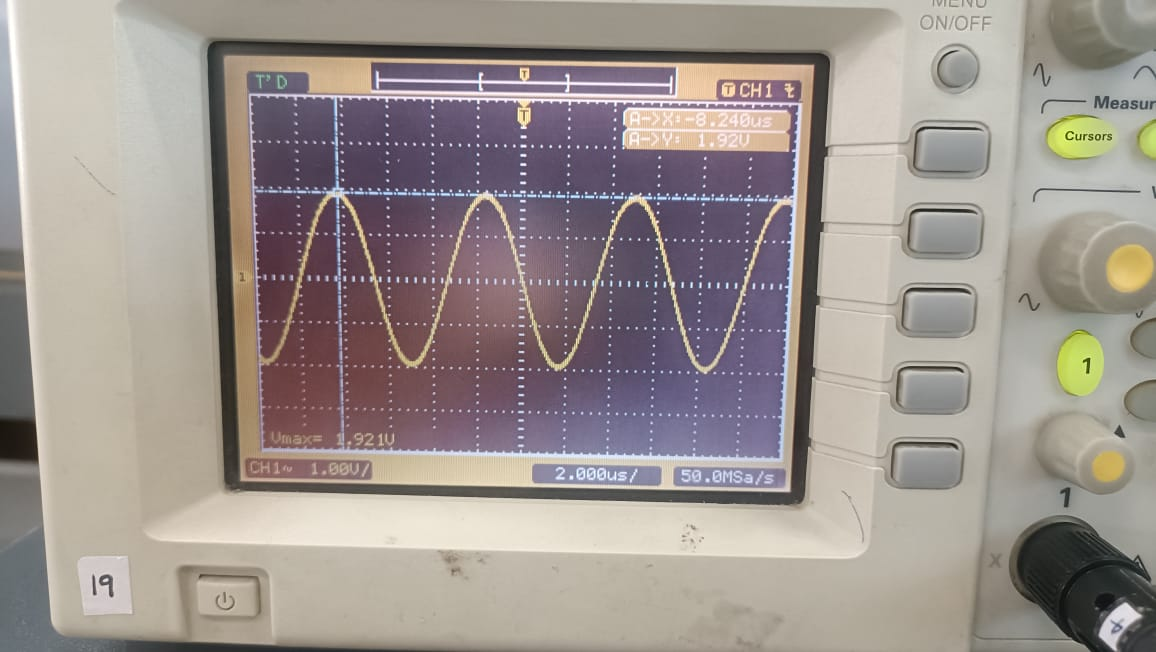
\includegraphics[width=0.7\textwidth]{figs/5.1/1.jpeg}
        \caption{$V_1=V_2=sin(2\pi ft)$ $f=150kHz$}
\end{figure}
\begin{figure}[H]
    \centering
    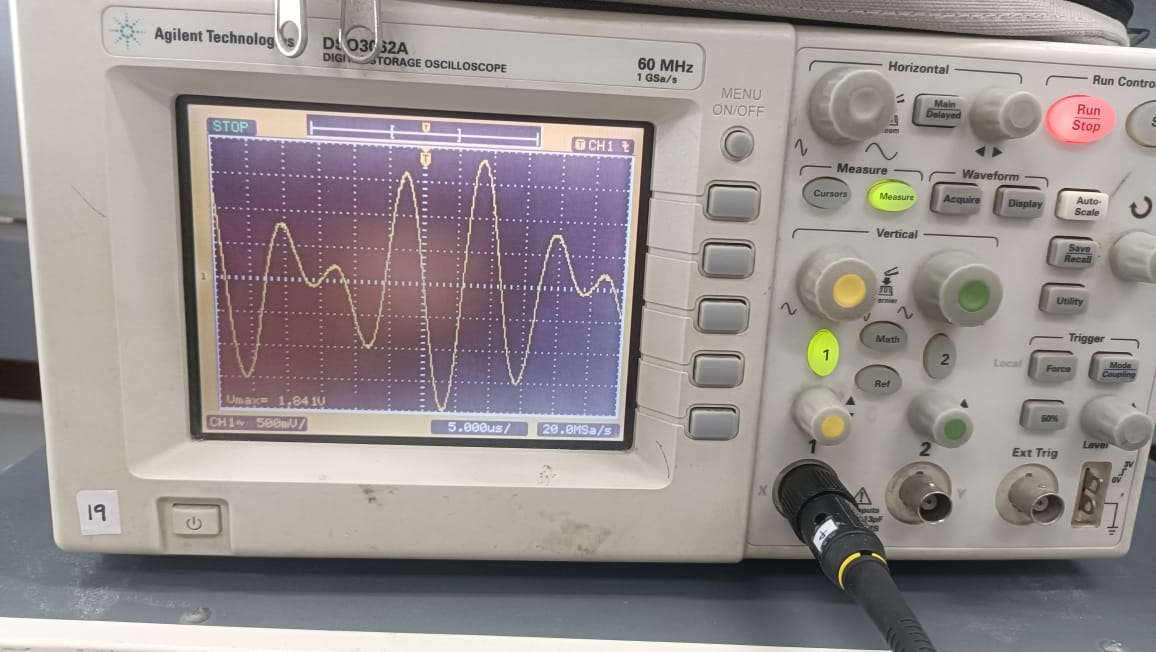
\includegraphics[width=0.7\textwidth]{figs/5.1/2.jpeg}
        \caption{$V_1=sin(2\pi f_1t), V_2=sin(2\pi f_2t), f_1=75kHz, f_2=100kHz$}
\end{figure}
\begin{figure}[H]
    \centering
    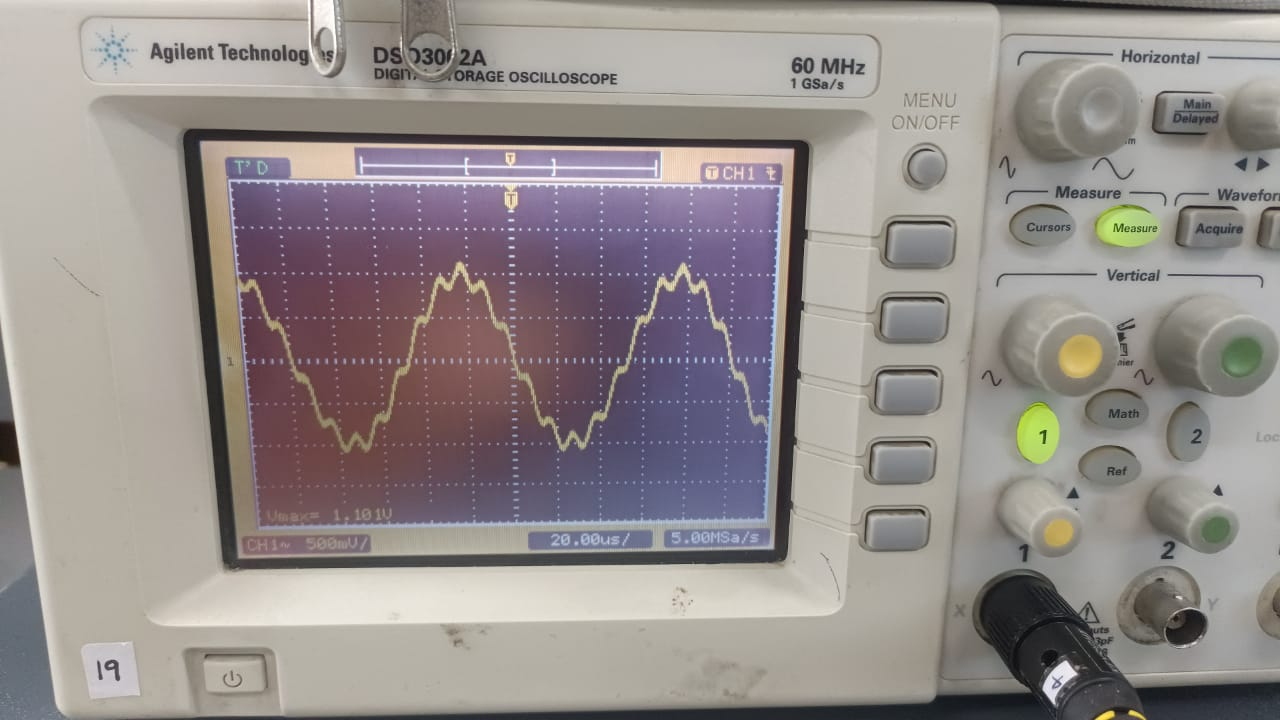
\includegraphics[width=0.7\textwidth]{figs/5.1/3.jpeg}
\end{figure}


\subsection*{Op-Amp Integrator}
\begin{figure}[H]
    \centering
    \begin{subfigure}{0.5\textwidth}
        \centering
        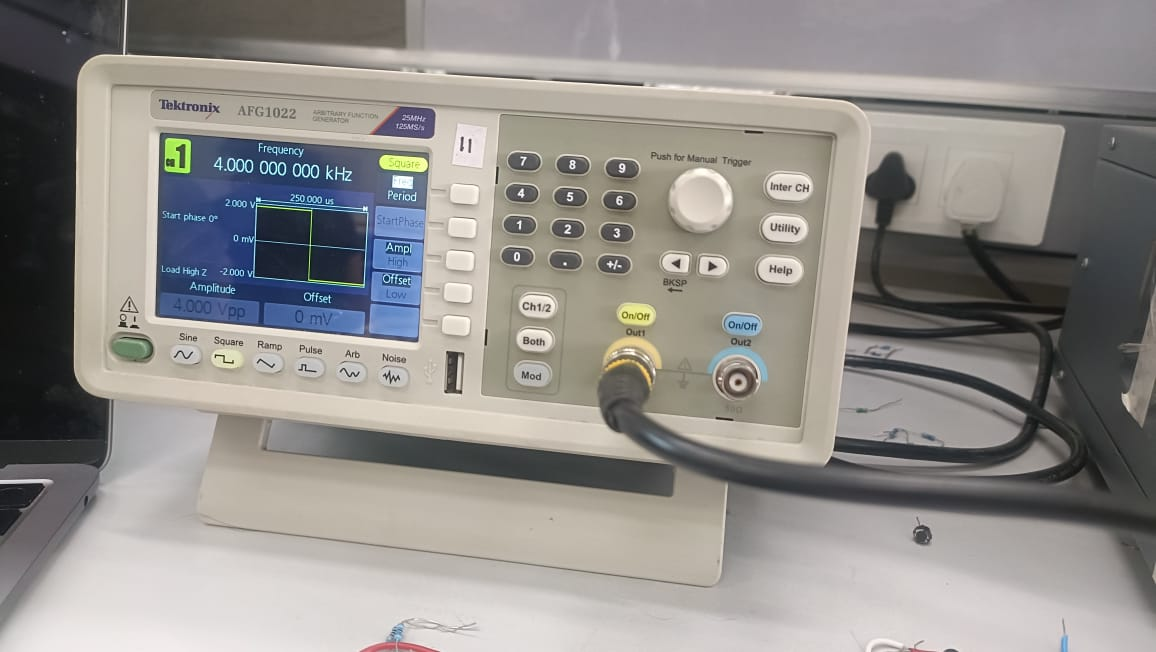
\includegraphics[height=5cm]{figs/5.2/para.jpeg}
    \end{subfigure}%
    \begin{subfigure}{0.5\textwidth}
        \centering
        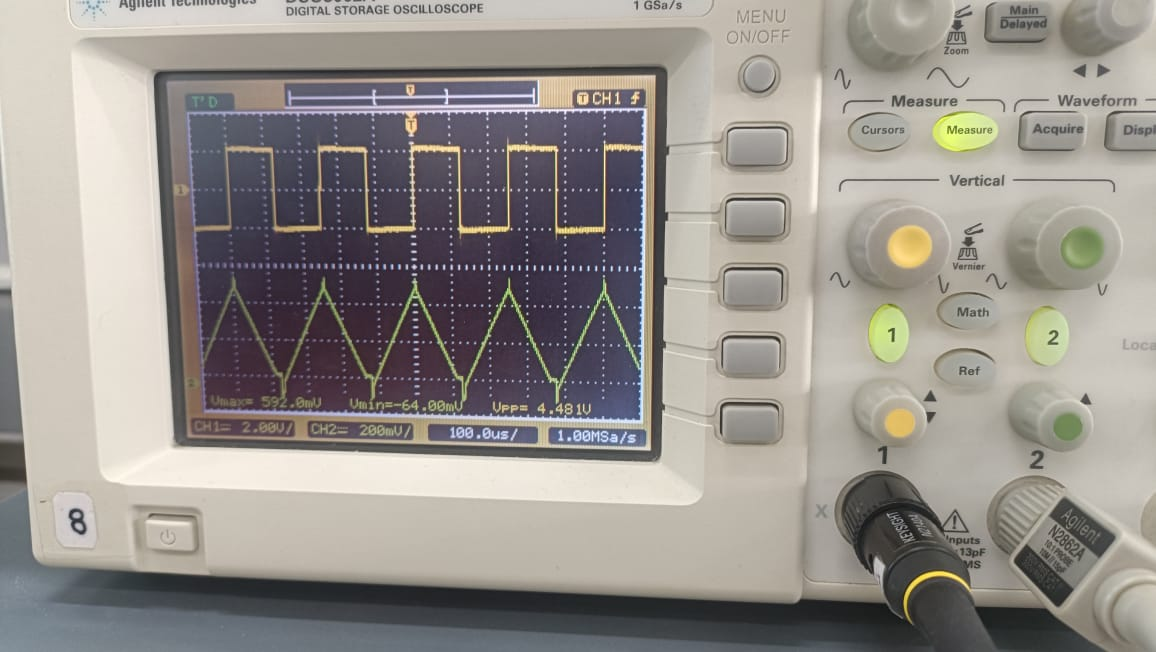
\includegraphics[height=5cm]{figs/5.2/plot.jpeg}
    \end{subfigure}
\end{figure}

\subsection*{Precision Rectifier}
\begin{figure}[H]
    \centering
    \begin{subfigure}{0.5\textwidth}
        \centering
        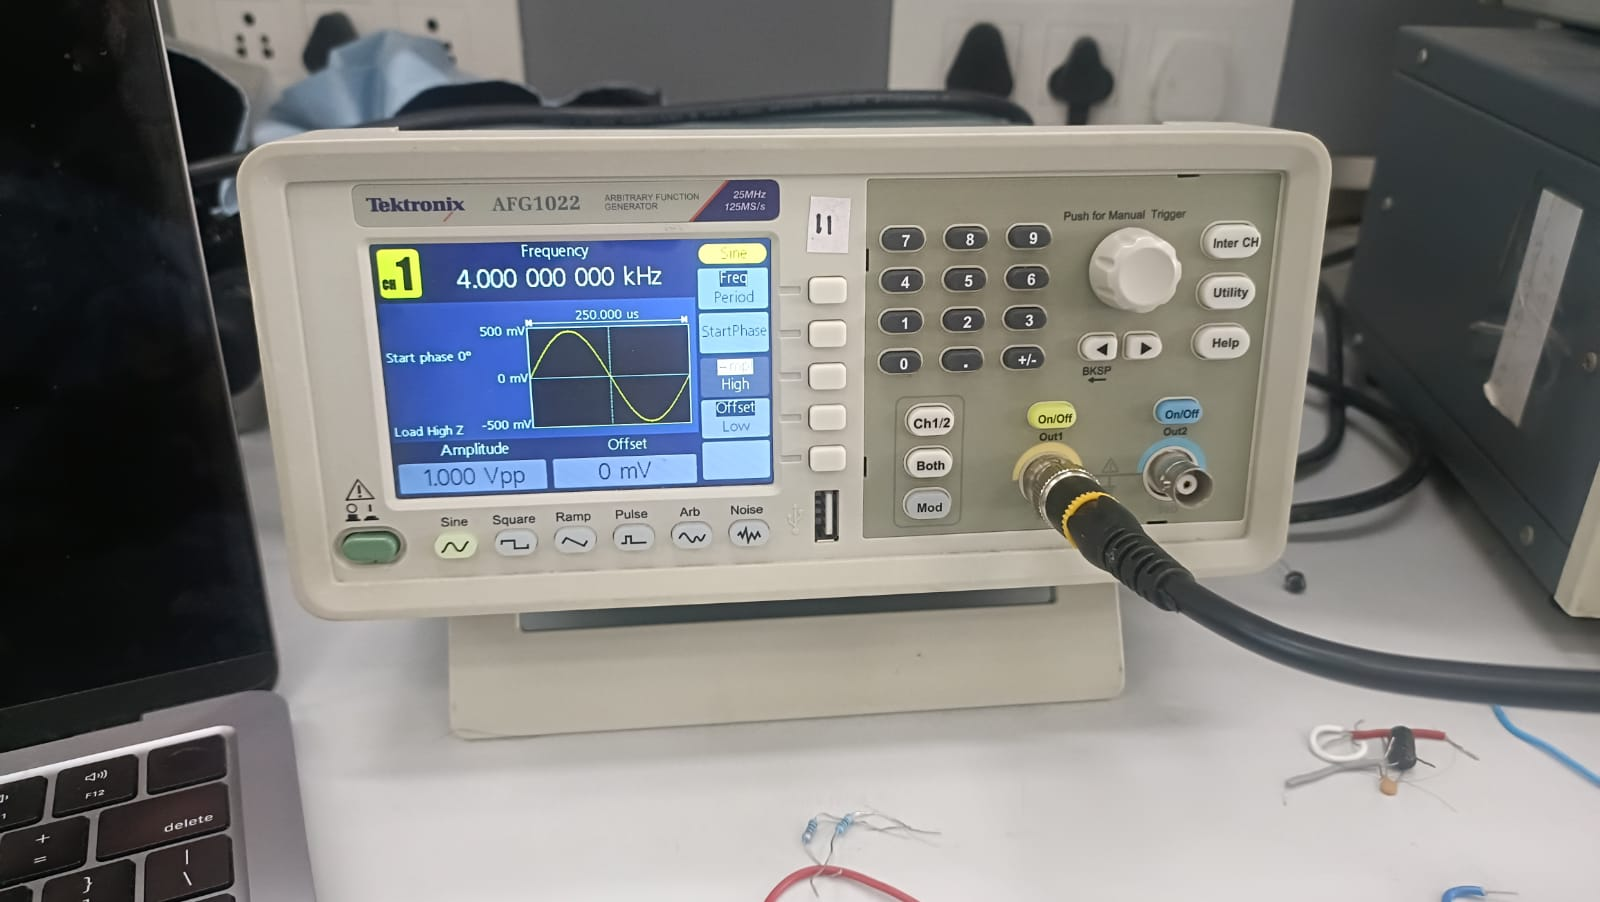
\includegraphics[height=5cm]{figs/5.3/para.jpeg}
    \end{subfigure}%
    \begin{subfigure}{0.5\textwidth}
        \centering
        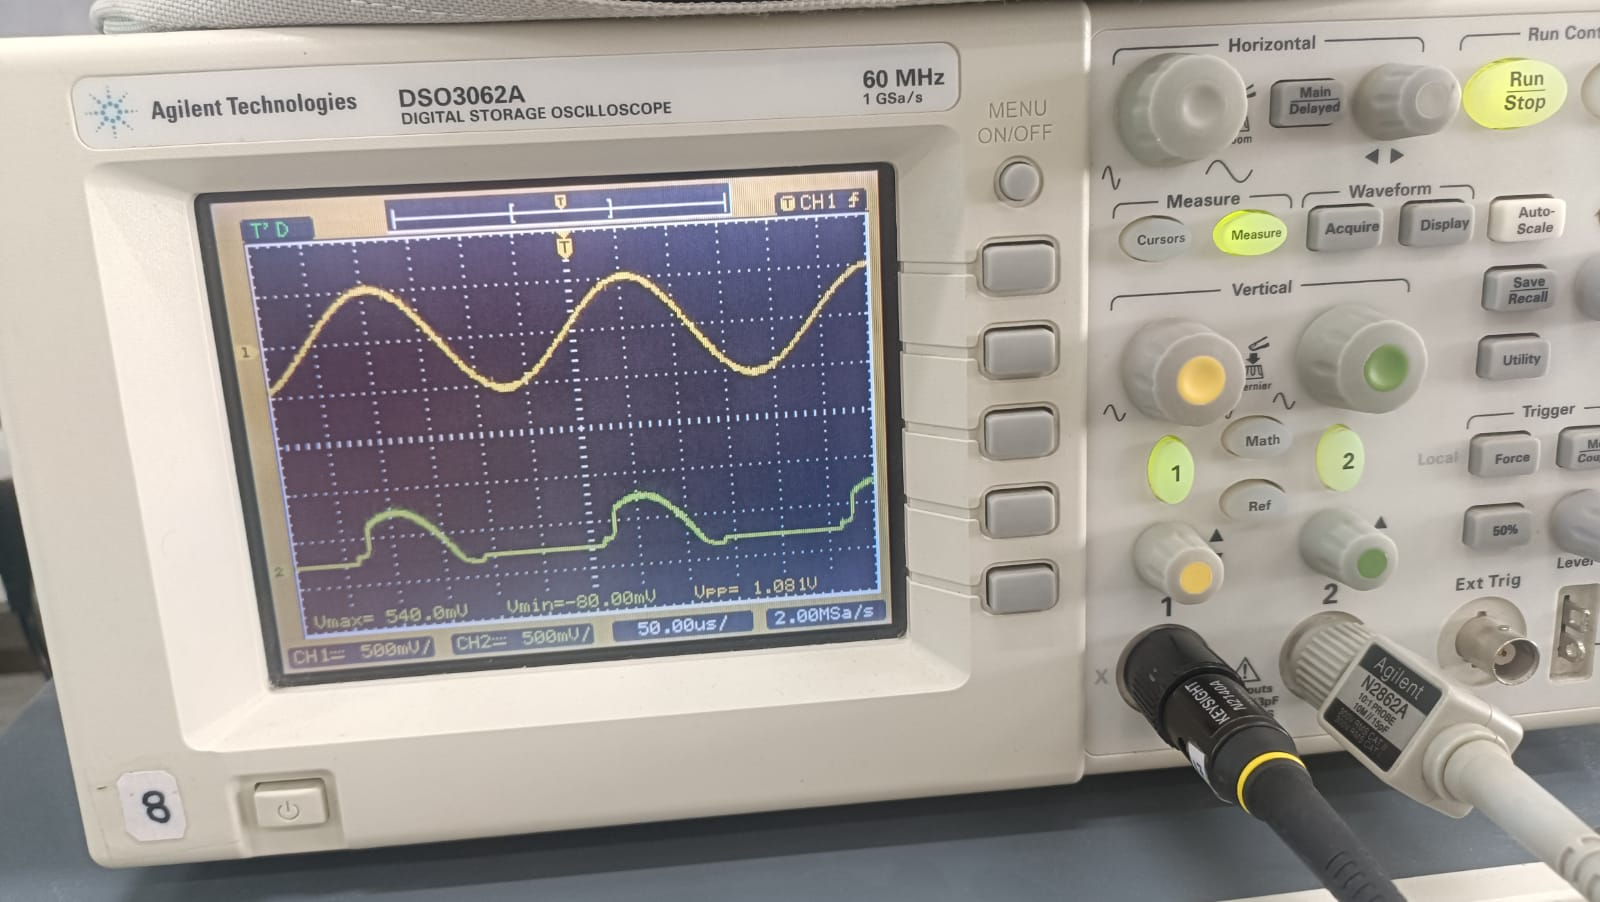
\includegraphics[height=5cm]{figs/5.3/plot.jpeg}
    \end{subfigure}
\end{figure}


\end{document}
